\chapter{Komponentenübergreifendes Systemverhalten im Nutzungskontext}

\begin{figure}[hbt]
  \centering
   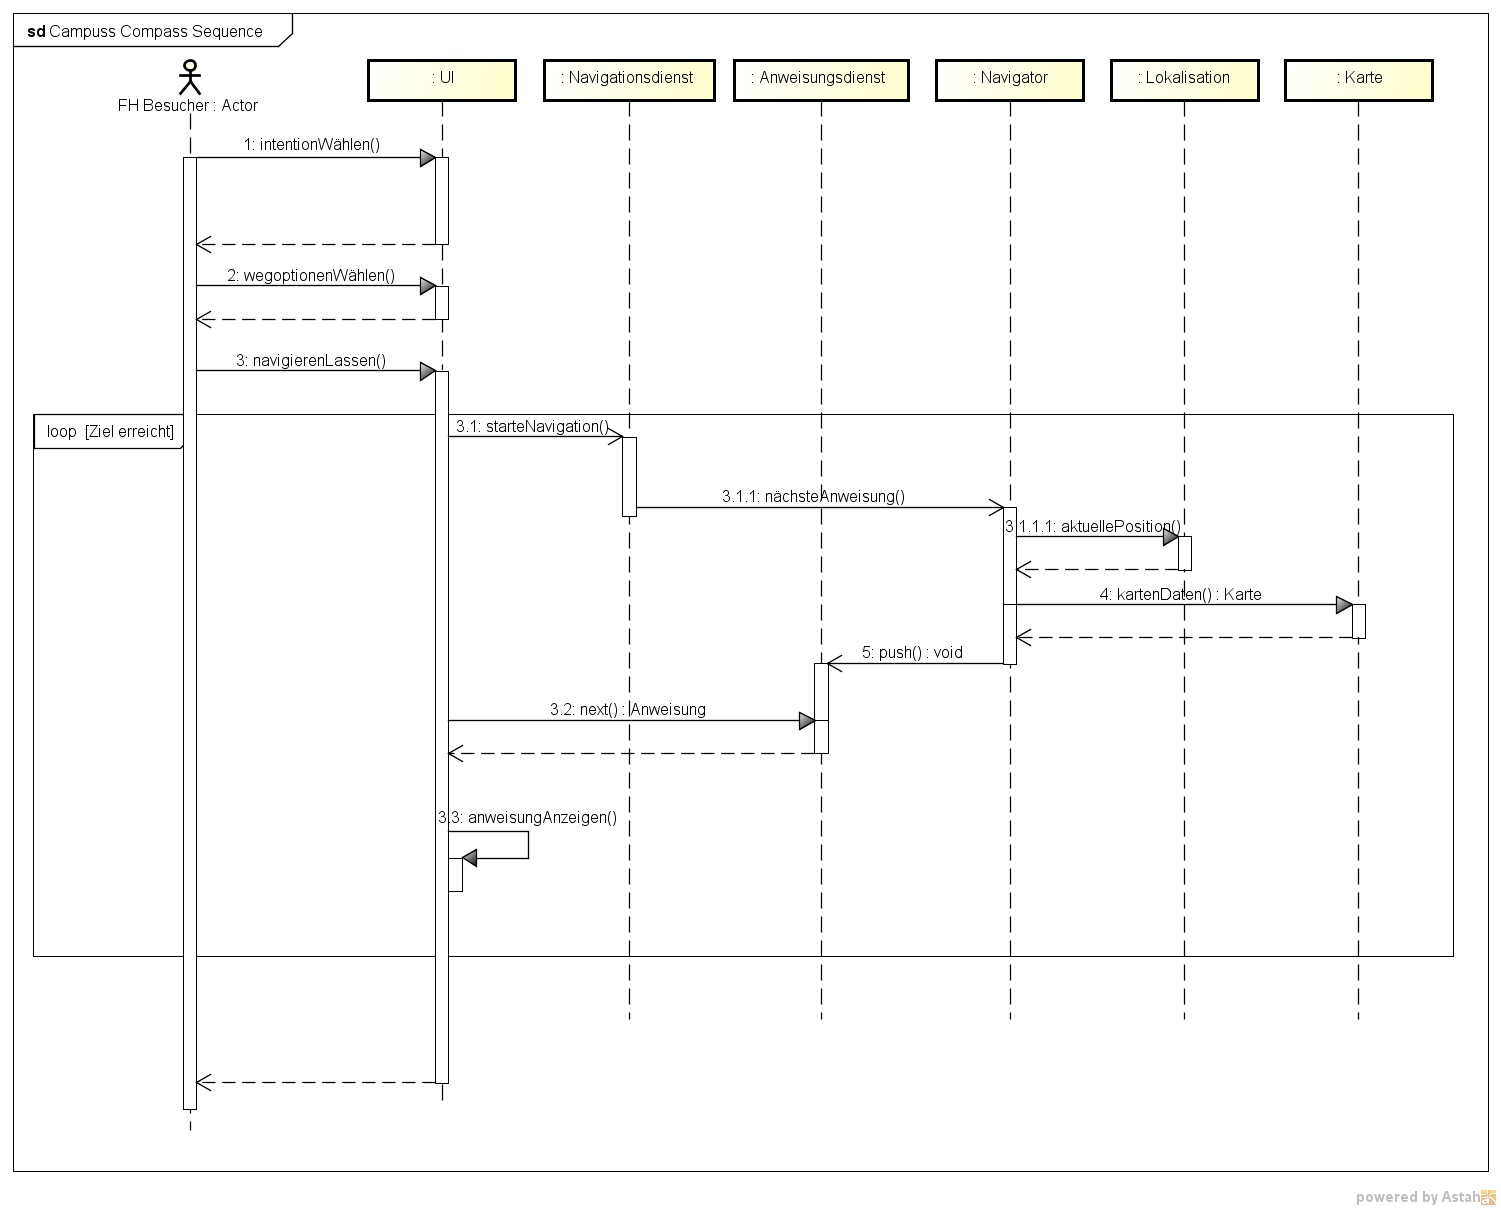
\includegraphics[width=\linewidth]{img/sequenzdiagramm.png}
  \caption{Sequenzdiagramm}
\label{fig:sequenzdiagramm}
\end{figure}

Das hier dargestelle Sequenzdiagramm beschreibt den Use-Case navigieren lassen.
Nachdem der User dem System seine Intention und Wegoptionen mitgeteilt hat,
tritt das System in einen Loop ein der erst verlassen wird wenn der User sein
Ziel erreicht hat.

\noindent Hierbei kommunizieren die einzelnen Komponenten des Systems
miteinander, um dem User den nächsten Schritt anzuzeigen.
